\documentclass[border=0pt]{standalone}
\usepackage{tikz}
\usetikzlibrary{calc,arrows.meta}

\definecolor{wallA}{HTML}{F1E3C9}
\definecolor{wallB}{HTML}{E2D0AE}
\definecolor{baseb}{HTML}{C9A97F}
\definecolor{floorA}{HTML}{B9834F}
\definecolor{floorB}{HTML}{99653A}
\definecolor{rugA}{HTML}{C5705C}
\definecolor{rugB}{HTML}{E0A183}
\definecolor{rugC}{HTML}{F3D9B7}
\definecolor{chairA}{HTML}{A85B4C}
\definecolor{chairB}{HTML}{8C463A}
\definecolor{chairC}{HTML}{C4715E}
\definecolor{woodA}{HTML}{8A5A3B}
\definecolor{woodB}{HTML}{6B4326}
\definecolor{skin}{HTML}{F3D3B5}
\definecolor{skinS}{HTML}{DFB292}
\definecolor{blush}{HTML}{E9A899}
\definecolor{hairA}{HTML}{EFEFEF}
\definecolor{hairB}{HTML}{CBCBCB}
\definecolor{cardi}{HTML}{B98BA5}
\definecolor{cardiS}{HTML}{9B7089}
\definecolor{skirt}{HTML}{5E7E86}
\definecolor{blankA}{HTML}{D98C6A}
\definecolor{blankB}{HTML}{F1BF9C}
\definecolor{tvbody}{HTML}{3B3B45}
\definecolor{tvdark}{HTML}{2A2A32}
\definecolor{tvscr}{HTML}{CDEBF8}
\definecolor{tvscr2}{HTML}{8CC7E8}
\definecolor{tvhill}{HTML}{6FA98C}
\definecolor{glow}{HTML}{FFF0BE}
\definecolor{lampA}{HTML}{F2C572}
\definecolor{lampB}{HTML}{D8A44E}
\definecolor{curt}{HTML}{E2A97E}
\definecolor{curtS}{HTML}{C4854D}
\definecolor{sky}{HTML}{2C3A5E}
\definecolor{skyL}{HTML}{47578A}
\definecolor{moonc}{HTML}{FBF0C4}
\definecolor{leaf}{HTML}{4F8B5B}
\definecolor{leafD}{HTML}{3B6B44}
\definecolor{potc}{HTML}{C4784E}
\definecolor{catc}{HTML}{D9A05B}
\definecolor{catd}{HTML}{B57F41}
\definecolor{cream}{HTML}{FBF3E2}

\begin{document}
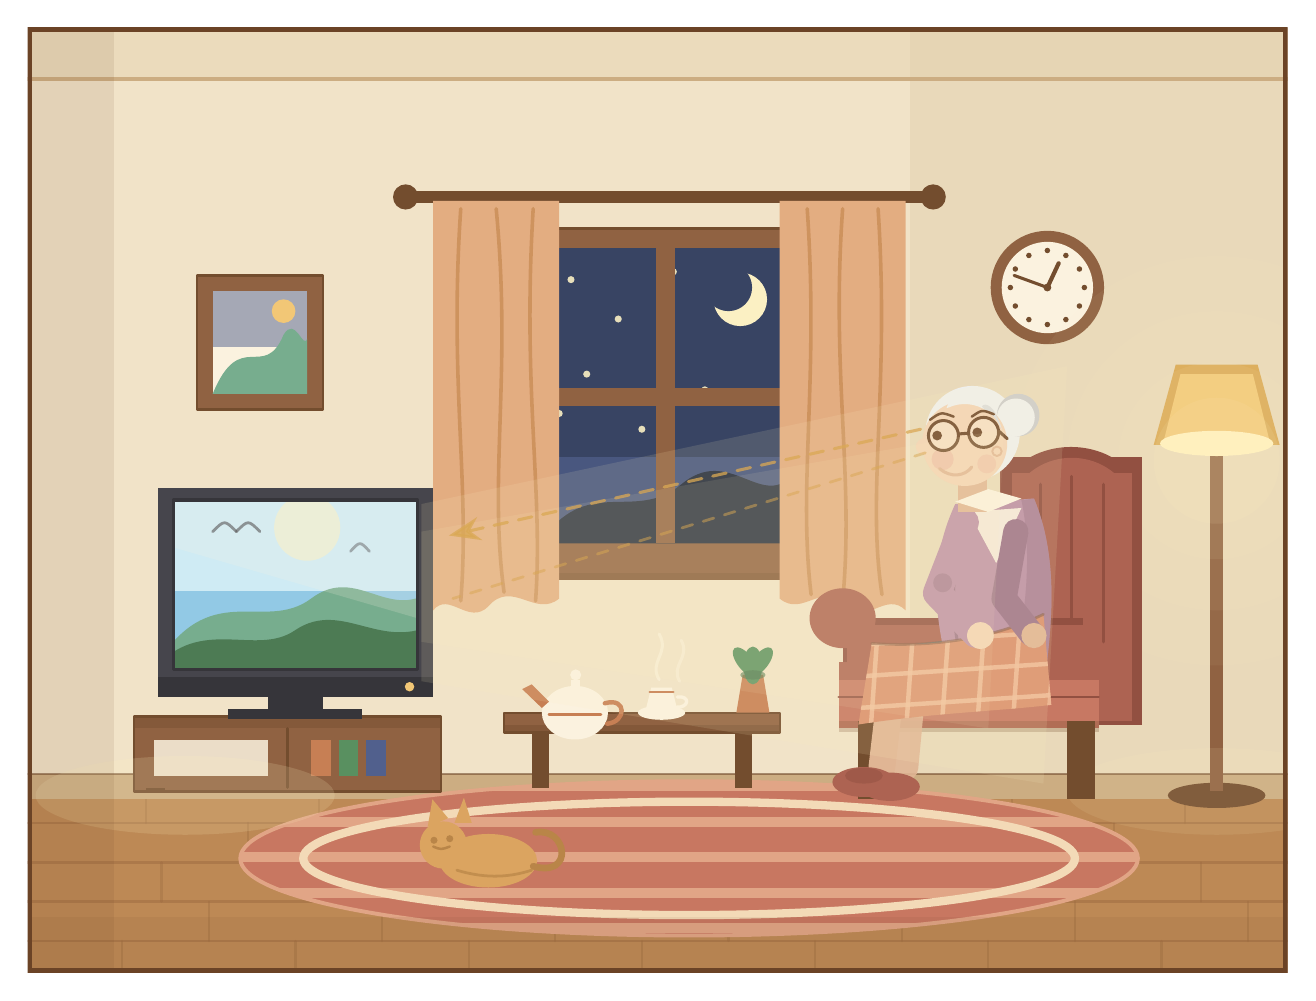
\begin{tikzpicture}[line join=round,line cap=round]
\clip (0,0) rectangle (16,12);

% ---------------- wall & floor ----------------
\fill[wallA] (0,2.2) rectangle (16,12);
\fill[wallB,opacity=0.55] (11.2,2.2) rectangle (16,12);
\fill[wallB,opacity=0.45] (0,11.35) rectangle (16,12);
\draw[baseb,line width=1.2pt] (0,11.35) -- (16,11.35);

\fill[floorA] (0,0) rectangle (16,2.2);
\foreach \y in {0.4,0.9,1.4,1.9}{\draw[floorB,line width=0.9pt,opacity=0.55] (0,\y) -- (16,\y);}
\foreach \x in {1.2,3.4,5.6,7.8,10.0,12.2,14.4}{\draw[floorB,line width=0.8pt,opacity=0.4] (\x,0) -- (\x,0.4);}
\foreach \x in {2.3,4.5,6.7,8.9,11.1,13.3,15.5}{\draw[floorB,line width=0.8pt,opacity=0.4] (\x,0.4) -- (\x,0.9);}
\foreach \x in {1.7,3.9,6.1,8.3,10.5,12.7,14.9}{\draw[floorB,line width=0.8pt,opacity=0.4] (\x,0.9) -- (\x,1.4);}
\foreach \x in {2.8,5.0,7.2,9.4,11.6,13.8}{\draw[floorB,line width=0.8pt,opacity=0.4] (\x,1.4) -- (\x,1.9);}
\foreach \x in {1.5,3.7,5.9,8.1,10.3,12.5,14.7}{\draw[floorB,line width=0.8pt,opacity=0.4] (\x,1.9) -- (\x,2.2);}

\fill[baseb] (0,2.2) rectangle (16,2.52);
\draw[woodB,line width=0.7pt,opacity=0.6] (0,2.52) -- (16,2.52);

% ---------------- rug ----------------
\begin{scope}
  \clip (8.4,1.45) ellipse (5.7 and 0.98);
  \fill[rugA] (2,0.2) rectangle (15,2.6);
  \foreach \y in {0.5,0.95,1.4,1.85,2.3}{\fill[rugB] (2,\y) rectangle (15,\y+0.13);}
  \draw[rugC,line width=3pt] (8.4,1.45) ellipse (4.9 and 0.72);
\end{scope}
\draw[rugB,line width=1.4pt] (8.4,1.45) ellipse (5.7 and 0.98);

% ---------------- window ----------------
\fill[woodA] (6.25,5.2) rectangle (9.95,9.45);
\fill[sky] (6.5,5.45) rectangle (9.7,9.2);
\fill[skyL,opacity=0.7] (6.5,5.45) rectangle (9.7,6.55);
\fill[moonc] (9.05,8.55) circle (0.34);
\fill[sky] (8.9,8.7) circle (0.3);
\foreach \p in {(6.9,8.8),(7.5,8.3),(7.1,7.6),(8.2,8.9),(6.75,7.1),(8.6,7.4),(7.8,6.9)}{\fill[moonc,opacity=0.9] \p circle (0.045);}
\fill[sky!60!black] (6.5,5.45) .. controls (7.1,6.35) and (7.7,5.7) .. (8.3,6.2) .. controls (8.9,6.7) and (9.3,5.9) .. (9.7,6.3) -- (9.7,5.45) -- cycle;
\fill[woodA] (7.98,5.45) rectangle (8.22,9.2);
\fill[woodA] (6.5,7.2) rectangle (9.7,7.42);
\draw[woodB,line width=1.1pt] (6.25,5.2) rectangle (9.95,9.45);
\fill[woodA] (6.0,4.98) rectangle (10.2,5.25);
\fill[woodB,opacity=0.35] (6.0,4.98) rectangle (10.2,5.08);

% ---------------- curtain rod & curtains ----------------
\draw[woodB,line width=4.5pt] (4.85,9.85) -- (11.45,9.85);
\fill[woodB] (4.8,9.85) circle (0.16);
\fill[woodB] (11.5,9.85) circle (0.16);

\fill[curt] (5.15,9.8) -- (6.75,9.8) -- (6.75,4.75) .. controls (6.45,4.5) and (6.15,5.0) .. (5.85,4.65)
  .. controls (5.6,4.4) and (5.35,4.85) .. (5.15,4.6) -- cycle;
\draw[curtS,line width=1.3pt,opacity=0.75] (5.5,9.7) .. controls (5.35,7.5) and (5.62,6.2) .. (5.5,4.72);
\draw[curtS,line width=1.3pt,opacity=0.75] (5.95,9.7) .. controls (6.15,7.6) and (5.85,6.3) .. (6.05,4.83);
\draw[curtS,line width=1.3pt,opacity=0.75] (6.42,9.7) .. controls (6.28,7.4) and (6.55,6.1) .. (6.45,4.72);

\fill[curt] (9.55,9.8) -- (11.15,9.8) -- (11.15,4.6) .. controls (10.9,4.85) and (10.65,4.4) .. (10.4,4.65)
  .. controls (10.1,5.0) and (9.85,4.5) .. (9.55,4.75) -- cycle;
\draw[curtS,line width=1.3pt,opacity=0.75] (9.9,9.7) .. controls (10.05,7.5) and (9.78,6.2) .. (9.95,4.8);
\draw[curtS,line width=1.3pt,opacity=0.75] (10.35,9.7) .. controls (10.2,7.6) and (10.5,6.3) .. (10.35,4.72);
\draw[curtS,line width=1.3pt,opacity=0.75] (10.8,9.7) .. controls (10.95,7.4) and (10.65,6.1) .. (10.85,4.8);

% ---------------- wall picture ----------------
\fill[woodA] (2.15,7.15) rectangle (3.75,8.85);
\fill[cream] (2.35,7.35) rectangle (3.55,8.65);
\fill[skyL,opacity=0.5] (2.35,7.95) rectangle (3.55,8.65);
\fill[tvhill] (2.35,7.35) .. controls (2.7,8.2) and (3.0,7.5) .. (3.25,8.1) .. controls (3.4,8.35) and (3.5,7.9) .. (3.55,8.05) -- (3.55,7.35) -- cycle;
\fill[lampA] (3.25,8.4) circle (0.15);
\draw[woodB,line width=0.9pt] (2.15,7.15) rectangle (3.75,8.85);

% ---------------- wall clock ----------------
\fill[woodA] (12.95,8.7) circle (0.72);
\fill[cream] (12.95,8.7) circle (0.58);
\foreach \a in {0,30,...,330}{\fill[woodB] (12.95,8.7) ++(\a:0.47) circle (0.035);}
\draw[woodB,line width=1.5pt] (12.95,8.7) -- ++(65:0.34);
\draw[woodB,line width=1.1pt] (12.95,8.7) -- ++(160:0.45);
\fill[woodB] (12.95,8.7) circle (0.05);

% ---------------- floor lamp ----------------
\fill[woodB] (15.1,2.25) ellipse (0.62 and 0.16);
\fill[woodA] (15.02,2.3) rectangle (15.18,6.7);
\fill[lampB] (14.3,6.7) -- (15.9,6.7) -- (15.62,7.72) -- (14.58,7.72) -- cycle;
\fill[lampA] (14.42,6.72) -- (15.78,6.72) -- (15.56,7.6) -- (14.64,7.6) -- cycle;
\fill[glow] (15.1,6.72) ellipse (0.72 and 0.16);
\foreach \r/\o in {2.6/0.05,1.9/0.06,1.25/0.08,0.8/0.10}{\fill[glow,opacity=\o] (15.1,6.5) circle (\r);}
\fill[glow,opacity=0.10] (15.1,2.3) ellipse (1.9 and 0.55);

% ---------------- TV stand & TV ----------------
\fill[woodA] (1.35,2.3) rectangle (5.25,3.25);
\fill[woodB,opacity=0.4] (1.35,3.1) rectangle (5.25,3.25);
\fill[woodB] (1.5,2.3) rectangle (1.75,2.35);
\draw[woodB,line width=0.9pt] (1.35,2.3) rectangle (5.25,3.25);
\draw[woodB,line width=0.9pt] (3.3,2.35) -- (3.3,3.1);
\fill[cream,opacity=0.85] (1.6,2.5) rectangle (3.05,2.95);
\fill[potc] (3.6,2.5) rectangle (3.85,2.95);
\fill[leaf] (3.95,2.5) rectangle (4.2,2.95);
\fill[skyL] (4.3,2.5) rectangle (4.55,2.95);

\fill[tvdark] (3.05,3.25) rectangle (3.75,3.55);
\fill[tvdark] (2.55,3.22) rectangle (4.25,3.35);
\fill[tvbody] (1.65,3.5) rectangle (5.15,6.15);
\fill[tvdark] (1.65,3.5) rectangle (5.15,3.75);
\begin{scope}
  \clip (1.85,3.85) rectangle (4.95,6.0);
  \fill[tvscr] (1.85,3.85) rectangle (4.95,6.0);
  \fill[tvscr2] (1.85,3.85) rectangle (4.95,4.85);
  \fill[glow,opacity=0.55] (3.55,5.65) circle (0.42);
  \fill[tvhill] (1.6,3.85) .. controls (2.3,5.05) and (3.0,4.3) .. (3.6,4.75) .. controls (4.2,5.2) and (4.6,4.4) .. (5.2,4.9) -- (5.2,3.85) -- cycle;
  \fill[leafD,opacity=0.85] (1.6,3.85) .. controls (2.2,4.55) and (2.9,4.0) .. (3.4,4.35) .. controls (4.0,4.75) and (4.5,4.05) .. (5.2,4.45) -- (5.2,3.85) -- cycle;
  \draw[tvdark,line width=1pt,opacity=0.6] (2.35,5.6) .. controls (2.5,5.75) .. (2.65,5.6);
  \draw[tvdark,line width=1pt,opacity=0.6] (2.65,5.6) .. controls (2.8,5.75) .. (2.95,5.6);
  \draw[tvdark,line width=1pt,opacity=0.45] (4.1,5.35) .. controls (4.22,5.48) .. (4.34,5.35);
  \fill[cream,opacity=0.18] (1.85,5.4) -- (4.95,4.5) -- (4.95,6.0) -- (1.85,6.0) -- cycle;
\end{scope}
\draw[tvdark,line width=1.2pt] (1.85,3.85) rectangle (4.95,6.0);
\fill[lampA] (4.85,3.63) circle (0.06);

% ---------------- coffee table ----------------
\fill[woodA] (6.05,3.05) rectangle (9.55,3.3);
\fill[woodB,opacity=0.45] (6.05,3.05) rectangle (9.55,3.14);
\fill[woodB] (6.4,2.35) rectangle (6.62,3.05);
\fill[woodB] (8.98,2.35) rectangle (9.2,3.05);
\draw[woodB,line width=0.8pt] (6.05,3.05) rectangle (9.55,3.3);

% teapot
\fill[cream] (6.95,3.3) ellipse (0.42 and 0.34);
\fill[cream] (6.95,3.6) rectangle (7.05,3.62);
\fill[cream] (6.9,3.6) rectangle (7.02,3.72);
\fill[cream] (6.96,3.78) circle (0.07);
\draw[potc,line width=1.6pt] (7.33,3.42) .. controls (7.62,3.5) and (7.6,3.18) .. (7.36,3.16);
\fill[potc] (6.53,3.36) -- (6.28,3.6) -- (6.4,3.66) -- (6.62,3.44) -- cycle;
\draw[potc,line width=1pt] (6.62,3.28) -- (7.28,3.28);

% cup
\fill[cream] (8.05,3.3) ellipse (0.3 and 0.09);
\fill[cream] (7.85,3.34) -- (8.25,3.34) -- (8.18,3.62) -- (7.92,3.62) -- cycle;
\draw[potc,line width=0.9pt] (7.9,3.56) -- (8.2,3.56);
\draw[cream,line width=1.2pt] (8.25,3.5) .. controls (8.42,3.52) and (8.4,3.36) .. (8.24,3.37);
\draw[cream,opacity=0.65,line width=1.1pt] (8.02,3.72) .. controls (7.88,3.95) and (8.16,4.05) .. (8.02,4.3);
\draw[cream,opacity=0.5,line width=1.1pt] (8.28,3.7) .. controls (8.16,3.9) and (8.42,4.0) .. (8.3,4.22);

% small plant on table
\fill[potc] (9.0,3.3) -- (9.42,3.3) -- (9.34,3.78) -- (9.08,3.78) -- cycle;
\fill[leaf] (9.21,3.9) ellipse (0.12 and 0.24);
\fill[leaf,rotate around={38:(9.21,3.82)}] (9.21,3.98) ellipse (0.1 and 0.22);
\fill[leaf,rotate around={-38:(9.21,3.82)}] (9.21,3.98) ellipse (0.1 and 0.22);
\fill[leafD,opacity=0.6] (9.21,3.78) ellipse (0.16 and 0.06);

% ---------------- armchair (back parts) ----------------
\fill[chairB] (12.35,3.15) rectangle (14.15,6.55);
\fill[chairB] (12.35,6.15) .. controls (12.7,6.85) and (13.8,6.85) .. (14.15,6.15) -- cycle;
\fill[chairA] (12.5,3.2) rectangle (14.02,6.35);
\fill[chairA] (12.5,6.05) .. controls (12.8,6.7) and (13.72,6.7) .. (14.02,6.05) -- cycle;
\draw[chairB,line width=1.2pt] (13.26,4.0) -- (13.26,6.3);
\draw[chairB,line width=1.2pt] (12.86,4.2) -- (12.86,6.2);
\draw[chairB,line width=1.2pt] (13.66,4.2) -- (13.66,6.2);
% far armrest
\fill[chairB] (10.35,3.75) rectangle (13.4,4.5);
\fill[chairA] (10.35,4.5) ellipse (0.42 and 0.38);
\fill[chairA] (10.4,3.85) rectangle (13.4,4.42);
% seat
\fill[chairC] (10.3,3.1) rectangle (13.6,3.95);
\fill[chairA] (10.3,3.72) rectangle (13.6,3.95);
\draw[chairB,line width=1pt] (10.3,3.5) -- (13.6,3.5);
% legs
\fill[woodB] (10.55,2.2) rectangle (10.9,3.2);
\fill[woodB] (13.2,2.2) rectangle (13.55,3.2);
\fill[woodB,opacity=0.25] (10.3,3.05) rectangle (13.6,3.2);

% ---------------- grandma ----------------
% legs
\draw[skirt,line width=0.48cm] (12.35,4.05) -- (11.0,3.9);
\draw[skinS,line width=0.34cm] (11.0,3.9) -- (10.85,2.62);
\draw[skirt,line width=0.44cm,opacity=0.85] (12.45,3.85) -- (11.25,3.66);
\draw[skinS,line width=0.32cm,opacity=0.9] (11.25,3.66) -- (11.15,2.6);
\fill[chairA] (10.62,2.42) ellipse (0.4 and 0.19);
\fill[chairA] (10.95,2.36) ellipse (0.38 and 0.18);
\fill[chairB,opacity=0.5] (10.62,2.5) ellipse (0.24 and 0.1);

% torso
\fill[cardi] (11.72,3.75) .. controls (11.45,4.7) and (11.5,5.35) .. (11.78,5.95)
  -- (12.78,6.02) .. controls (13.08,5.3) and (13.02,4.5) .. (12.92,3.75) -- cycle;
\fill[cardiS,opacity=0.55] (12.5,3.78) .. controls (12.7,4.6) and (12.75,5.4) .. (12.62,6.0)
  -- (12.78,6.02) .. controls (13.08,5.3) and (13.02,4.5) .. (12.92,3.75) -- cycle;
\draw[cardiS,line width=1.1pt] (11.86,5.9) .. controls (11.72,5.0) and (11.72,4.4) .. (11.9,3.8);
\fill[cream,opacity=0.9] (11.95,5.85) -- (12.3,5.2) -- (12.62,5.9) -- cycle;

% blanket over lap
\fill[blankA] (12.9,4.55) .. controls (12.35,4.28) and (11.6,4.12) .. (10.72,4.18)
  -- (10.55,3.15) .. controls (11.5,3.3) and (12.35,3.32) .. (13.0,3.4) -- cycle;
\begin{scope}
  \clip (12.9,4.55) .. controls (12.35,4.28) and (11.6,4.12) .. (10.72,4.18)
    -- (10.55,3.15) .. controls (11.5,3.3) and (12.35,3.32) .. (13.0,3.4) -- cycle;
  \foreach \x in {10.7,11.15,11.6,12.05,12.5,12.95}{\draw[blankB,line width=1.6pt,opacity=0.8] (\x,3.0) -- (\x+0.12,4.7);}
  \foreach \y in {3.35,3.75,4.15}{\draw[blankB,line width=1.6pt,opacity=0.8] (10.4,\y) -- (13.1,\y+0.18);}
\end{scope}
\draw[blankA!60!black,line width=1pt,opacity=0.6] (12.9,4.55) .. controls (12.35,4.28) and (11.6,4.12) .. (10.72,4.18);

% arms
\draw[cardiS,line width=0.32cm] (12.55,5.6) -- (12.4,4.75) -- (12.75,4.3);
\fill[skinS] (12.78,4.28) circle (0.16);
\draw[cardi,line width=0.36cm] (11.9,5.72) -- (11.55,4.82) -- (12.05,4.3);
\fill[skin] (12.1,4.28) circle (0.17);
\fill[cardiS,opacity=0.6] (11.62,4.95) circle (0.12);

% neck & head
\fill[skinS] (11.82,5.85) rectangle (12.18,6.35);
\fill[hairA] (12.0,6.85) circle (0.6);
\fill[hairB] (12.58,7.08) circle (0.27);
\fill[hairA] (12.55,7.05) circle (0.24);
\fill[skin] (11.9,6.72) circle (0.54);
\fill[skin] (11.38,6.68) circle (0.1);
\fill[skin] (12.3,6.62) circle (0.12);
\draw[skinS,line width=0.7pt] (12.31,6.62) circle (0.06);
\fill[hairA] (11.9,6.72) ++(115:0.5) arc (115:20:0.5) .. controls (12.28,7.35) and (11.72,7.42) .. (11.67,7.17) -- cycle;
\fill[hairB,opacity=0.5] (11.9,6.72) ++(60:0.5) arc (60:22:0.5) .. controls (12.3,7.2) and (12.15,7.25) .. (12.12,7.19) -- cycle;
% blush
\fill[blush,opacity=0.45] (11.62,6.52) circle (0.14);
\fill[blush,opacity=0.35] (12.18,6.46) circle (0.12);
% glasses
\draw[woodB,line width=1.1pt] (11.63,6.82) circle (0.19);
\draw[woodB,line width=1.1pt] (12.14,6.86) circle (0.19);
\draw[woodB,line width=1.1pt] (11.82,6.84) -- (11.95,6.85);
\draw[woodB,line width=1.1pt] (12.33,6.88) -- (12.44,6.78);
\fill[cream,opacity=0.35] (11.63,6.82) circle (0.17);
\fill[cream,opacity=0.35] (12.14,6.86) circle (0.17);
% eyes looking left toward the TV
\fill[woodB] (11.55,6.82) circle (0.062);
\fill[woodB] (12.06,6.86) circle (0.062);
\draw[woodB,line width=0.9pt] (11.46,7.02) .. controls (11.6,7.12) .. (11.76,7.06);
\draw[woodB,line width=0.9pt] (11.99,7.06) .. controls (12.12,7.15) .. (12.27,7.09);
% smile
\draw[skinS,line width=1.1pt] (11.58,6.4) .. controls (11.72,6.28) and (11.9,6.3) .. (11.99,6.42);
% collar
\fill[cream] (11.78,5.98) -- (12.2,5.85) -- (12.62,6.02) -- (12.2,6.14) -- cycle;

% ---------------- cat on the rug ----------------
\fill[catc] (5.85,1.42) ellipse (0.62 and 0.34);
\fill[catc] (5.28,1.62) circle (0.3);
\fill[catc] (5.08,1.85) -- (5.14,2.2) -- (5.34,1.96) -- cycle;
\fill[catc] (5.42,1.9) -- (5.54,2.22) -- (5.64,1.9) -- cycle;
\draw[catd,line width=2.4pt] (6.42,1.35) .. controls (6.95,1.2) and (6.85,1.85) .. (6.45,1.78);
\draw[catd,line width=0.9pt] (5.15,1.6) .. controls (5.25,1.56) .. (5.36,1.6);
\fill[catd] (5.16,1.68) circle (0.045);
\fill[catd] (5.36,1.7) circle (0.045);
\draw[catd,line width=1pt,opacity=0.7] (5.45,1.3) .. controls (5.85,1.18) and (6.15,1.22) .. (6.4,1.3);

% ---------------- TV light spilling into the room ----------------
\fill[glow,opacity=0.13] (5.0,5.95) -- (13.2,7.7) -- (12.9,2.4) -- (5.0,3.7) -- cycle;
\fill[glow,opacity=0.10] (5.0,5.6) -- (12.4,6.9) -- (12.2,3.1) -- (5.0,4.2) -- cycle;
\fill[glow,opacity=0.16] (2.0,2.25) ellipse (1.9 and 0.5);

% ---------------- gaze toward the TV ----------------
\draw[lampB,opacity=0.75,line width=1.1pt,dash pattern=on 5pt off 4pt,-{Stealth[length=4mm,width=3mm]}]
  (11.34,6.9) -- (5.35,5.55);
\draw[lampB,opacity=0.5,line width=1.0pt,dash pattern=on 4pt off 4pt]
  (11.4,6.6) -- (5.4,4.75);

% ---------------- final warm ambience ----------------
\fill[glow,opacity=0.06] (0,0) rectangle (16,12);
\fill[woodB,opacity=0.10] (0,0) rectangle (1.1,12);
\fill[woodB,opacity=0.08] (0,0) rectangle (16,0.7);

\draw[woodB,line width=3pt] (0,0) rectangle (16,12);
\end{tikzpicture}
\end{document}
